\documentclass[border=10pt]{standalone}
\usepackage{tikz}
\usetikzlibrary{positioning,arrows.meta,calc,fit,patterns}

\begin{document}
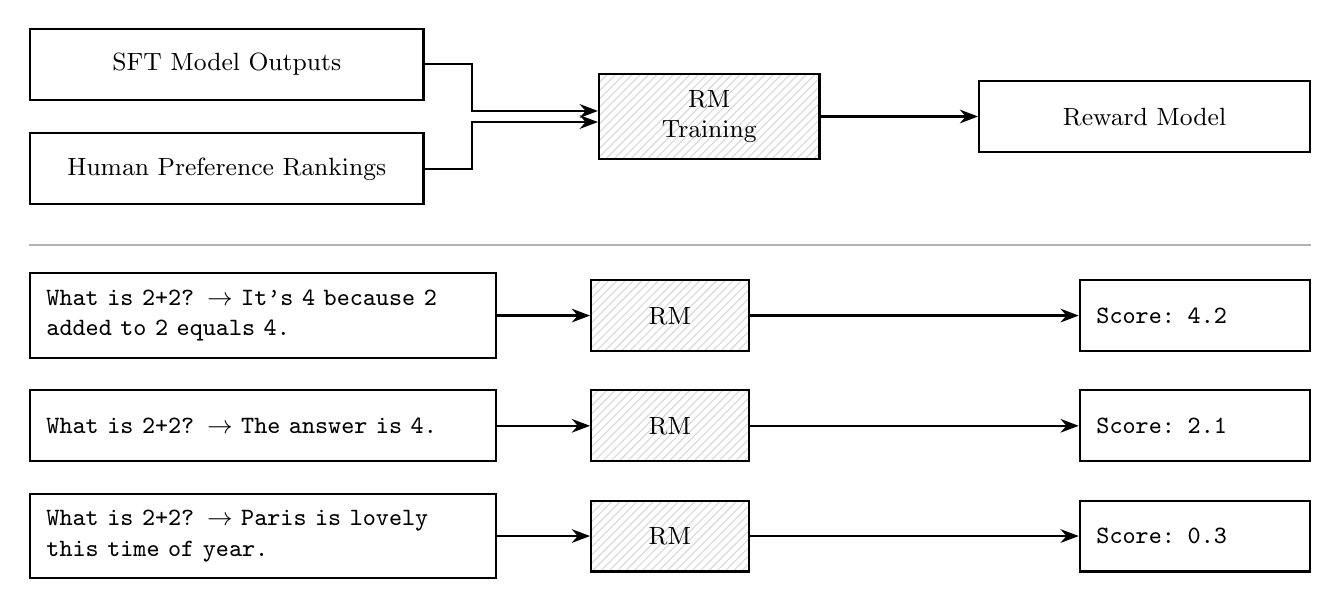
\begin{tikzpicture}[
    >=Stealth,
    every node/.style={font=\small},
    box/.style={draw, thick, minimum height=0.9cm, inner sep=6pt, text centered},
    inputbox/.style={box, fill=white, align=left},
    outputbox/.style={box, fill=white, align=left},
    modelbox/.style={box, pattern=north east lines, pattern color=black!15, minimum width=2.0cm, minimum height=0.9cm, align=center},
    flowbox/.style={box, fill=white, minimum width=3.6cm},
    flowarrow/.style={->, thick, black},
]

% ---- Top: Process Flow ----
\node[flowbox, minimum width=5.0cm] (sftouts) {SFT Model Outputs};
\node[flowbox, minimum width=5.0cm, below=0.4cm of sftouts] (prefs) {Human Preference Rankings};
\node[modelbox, right=2.2cm of $(sftouts.east)!0.5!(prefs.east)$, minimum width=2.8cm] (rmtrain) {RM\\Training};
\node[flowbox, minimum width=4.2cm, right=2.0cm of rmtrain] (rmmodel) {Reward Model};

% Arrows from both inputs enter RM Training at different heights
\draw[flowarrow] (sftouts.east) -- ++(0.6cm,0) |- ([yshift=2pt]rmtrain.west);
\draw[flowarrow] (prefs.east) -- ++(0.6cm,0) |- ([yshift=-2pt]rmtrain.west);
\draw[flowarrow] (rmtrain) -- (rmmodel);

% ---- Divider ----
\coordinate (leftedge) at (sftouts.west);
\coordinate (rightedge) at (rmmodel.east);
\draw[thick, black!30] ([yshift=-0.5cm]leftedge |- prefs.south) -- ([yshift=-0.5cm]rightedge |- prefs.south);

% ---- Bottom: Example I/O ----
\coordinate (figcenter) at ($(leftedge)!0.5!(rightedge)$);

\coordinate (row1) at ([yshift=-1.4cm]prefs.south -| figcenter);
\coordinate (row2) at ([yshift=-1.4cm]row1);
\coordinate (row3) at ([yshift=-1.4cm]row2);

% Place RM boxes at the true center
\node[modelbox, minimum width=2.0cm] (m1) at (row1) {RM};
\node[modelbox, minimum width=2.0cm] (m2) at (row2) {RM};
\node[modelbox, minimum width=2.0cm] (m3) at (row3) {RM};

% Row 1
\node[inputbox, text width=5.5cm, anchor=west] (in1) at (leftedge |- row1) {\texttt{What is 2+2? $\rightarrow$ It's 4 because 2 added to 2 equals 4.}};
\node[outputbox, text width=2.5cm, anchor=east] (out1) at (rightedge |- row1) {\texttt{Score: 4.2}};
\draw[flowarrow] (in1) -- (m1);
\draw[flowarrow] (m1) -- (out1);

% Row 2
\node[inputbox, text width=5.5cm, anchor=west] (in2) at (leftedge |- row2) {\texttt{What is 2+2? $\rightarrow$ The answer is 4.}};
\node[outputbox, text width=2.5cm, anchor=east] (out2) at (rightedge |- row2) {\texttt{Score: 2.1}};
\draw[flowarrow] (in2) -- (m2);
\draw[flowarrow] (m2) -- (out2);

% Row 3
\node[inputbox, text width=5.5cm, anchor=west] (in3) at (leftedge |- row3) {\texttt{What is 2+2? $\rightarrow$ Paris is lovely this time of year.}};
\node[outputbox, text width=2.5cm, anchor=east] (out3) at (rightedge |- row3) {\texttt{Score: 0.3}};
\draw[flowarrow] (in3) -- (m3);
\draw[flowarrow] (m3) -- (out3);

\end{tikzpicture}
\end{document}
